\documentclass[]{article}
\usepackage{lmodern}
\usepackage{amssymb,amsmath}
\usepackage{ifxetex,ifluatex}
\usepackage{fixltx2e} % provides \textsubscript
\ifnum 0\ifxetex 1\fi\ifluatex 1\fi=0 % if pdftex
  \usepackage[T1]{fontenc}
  \usepackage[utf8]{inputenc}
\else % if luatex or xelatex
  \ifxetex
    \usepackage{mathspec}
  \else
    \usepackage{fontspec}
  \fi
  \defaultfontfeatures{Ligatures=TeX,Scale=MatchLowercase}
\fi
% use upquote if available, for straight quotes in verbatim environments
\IfFileExists{upquote.sty}{\usepackage{upquote}}{}
% use microtype if available
\IfFileExists{microtype.sty}{%
\usepackage{microtype}
\UseMicrotypeSet[protrusion]{basicmath} % disable protrusion for tt fonts
}{}
\usepackage[margin=0.25in]{geometry}
\usepackage{hyperref}
\hypersetup{unicode=true,
            pdftitle={STAT565\_Lab},
            pdfauthor={Shen Qu},
            pdfborder={0 0 0},
            breaklinks=true}
\urlstyle{same}  % don't use monospace font for urls
\usepackage{color}
\usepackage{fancyvrb}
\newcommand{\VerbBar}{|}
\newcommand{\VERB}{\Verb[commandchars=\\\{\}]}
\DefineVerbatimEnvironment{Highlighting}{Verbatim}{commandchars=\\\{\}}
% Add ',fontsize=\small' for more characters per line
\usepackage{framed}
\definecolor{shadecolor}{RGB}{248,248,248}
\newenvironment{Shaded}{\begin{snugshade}}{\end{snugshade}}
\newcommand{\AlertTok}[1]{\textcolor[rgb]{0.94,0.16,0.16}{#1}}
\newcommand{\AnnotationTok}[1]{\textcolor[rgb]{0.56,0.35,0.01}{\textbf{\textit{#1}}}}
\newcommand{\AttributeTok}[1]{\textcolor[rgb]{0.77,0.63,0.00}{#1}}
\newcommand{\BaseNTok}[1]{\textcolor[rgb]{0.00,0.00,0.81}{#1}}
\newcommand{\BuiltInTok}[1]{#1}
\newcommand{\CharTok}[1]{\textcolor[rgb]{0.31,0.60,0.02}{#1}}
\newcommand{\CommentTok}[1]{\textcolor[rgb]{0.56,0.35,0.01}{\textit{#1}}}
\newcommand{\CommentVarTok}[1]{\textcolor[rgb]{0.56,0.35,0.01}{\textbf{\textit{#1}}}}
\newcommand{\ConstantTok}[1]{\textcolor[rgb]{0.00,0.00,0.00}{#1}}
\newcommand{\ControlFlowTok}[1]{\textcolor[rgb]{0.13,0.29,0.53}{\textbf{#1}}}
\newcommand{\DataTypeTok}[1]{\textcolor[rgb]{0.13,0.29,0.53}{#1}}
\newcommand{\DecValTok}[1]{\textcolor[rgb]{0.00,0.00,0.81}{#1}}
\newcommand{\DocumentationTok}[1]{\textcolor[rgb]{0.56,0.35,0.01}{\textbf{\textit{#1}}}}
\newcommand{\ErrorTok}[1]{\textcolor[rgb]{0.64,0.00,0.00}{\textbf{#1}}}
\newcommand{\ExtensionTok}[1]{#1}
\newcommand{\FloatTok}[1]{\textcolor[rgb]{0.00,0.00,0.81}{#1}}
\newcommand{\FunctionTok}[1]{\textcolor[rgb]{0.00,0.00,0.00}{#1}}
\newcommand{\ImportTok}[1]{#1}
\newcommand{\InformationTok}[1]{\textcolor[rgb]{0.56,0.35,0.01}{\textbf{\textit{#1}}}}
\newcommand{\KeywordTok}[1]{\textcolor[rgb]{0.13,0.29,0.53}{\textbf{#1}}}
\newcommand{\NormalTok}[1]{#1}
\newcommand{\OperatorTok}[1]{\textcolor[rgb]{0.81,0.36,0.00}{\textbf{#1}}}
\newcommand{\OtherTok}[1]{\textcolor[rgb]{0.56,0.35,0.01}{#1}}
\newcommand{\PreprocessorTok}[1]{\textcolor[rgb]{0.56,0.35,0.01}{\textit{#1}}}
\newcommand{\RegionMarkerTok}[1]{#1}
\newcommand{\SpecialCharTok}[1]{\textcolor[rgb]{0.00,0.00,0.00}{#1}}
\newcommand{\SpecialStringTok}[1]{\textcolor[rgb]{0.31,0.60,0.02}{#1}}
\newcommand{\StringTok}[1]{\textcolor[rgb]{0.31,0.60,0.02}{#1}}
\newcommand{\VariableTok}[1]{\textcolor[rgb]{0.00,0.00,0.00}{#1}}
\newcommand{\VerbatimStringTok}[1]{\textcolor[rgb]{0.31,0.60,0.02}{#1}}
\newcommand{\WarningTok}[1]{\textcolor[rgb]{0.56,0.35,0.01}{\textbf{\textit{#1}}}}
\usepackage{longtable,booktabs}
\usepackage{graphicx,grffile}
\makeatletter
\def\maxwidth{\ifdim\Gin@nat@width>\linewidth\linewidth\else\Gin@nat@width\fi}
\def\maxheight{\ifdim\Gin@nat@height>\textheight\textheight\else\Gin@nat@height\fi}
\makeatother
% Scale images if necessary, so that they will not overflow the page
% margins by default, and it is still possible to overwrite the defaults
% using explicit options in \includegraphics[width, height, ...]{}
\setkeys{Gin}{width=\maxwidth,height=\maxheight,keepaspectratio}
\IfFileExists{parskip.sty}{%
\usepackage{parskip}
}{% else
\setlength{\parindent}{0pt}
\setlength{\parskip}{6pt plus 2pt minus 1pt}
}
\setlength{\emergencystretch}{3em}  % prevent overfull lines
\providecommand{\tightlist}{%
  \setlength{\itemsep}{0pt}\setlength{\parskip}{0pt}}
\setcounter{secnumdepth}{0}
% Redefines (sub)paragraphs to behave more like sections
\ifx\paragraph\undefined\else
\let\oldparagraph\paragraph
\renewcommand{\paragraph}[1]{\oldparagraph{#1}\mbox{}}
\fi
\ifx\subparagraph\undefined\else
\let\oldsubparagraph\subparagraph
\renewcommand{\subparagraph}[1]{\oldsubparagraph{#1}\mbox{}}
\fi

%%% Use protect on footnotes to avoid problems with footnotes in titles
\let\rmarkdownfootnote\footnote%
\def\footnote{\protect\rmarkdownfootnote}

%%% Change title format to be more compact
\usepackage{titling}

% Create subtitle command for use in maketitle
\newcommand{\subtitle}[1]{
  \posttitle{
    \begin{center}\large#1\end{center}
    }
}

\setlength{\droptitle}{-2em}

  \title{STAT565\_Lab}
    \pretitle{\vspace{\droptitle}\centering\huge}
  \posttitle{\par}
    \author{Shen Qu}
    \preauthor{\centering\large\emph}
  \postauthor{\par}
      \predate{\centering\large\emph}
  \postdate{\par}
    \date{Mar 11, 2019}


\begin{document}
\maketitle

\begin{enumerate}
\def\labelenumi{(\alph{enumi})}
\tightlist
\item
  \textcolor[rgb]{0.5,0.5,0.5}{Plot the data and report the plot here (A plot with data and means of treatment combinations). Do not report code here. Describe the observed relationship between two factors.}
\end{enumerate}

\begin{verbatim}
## Classes 'tbl_df', 'tbl' and 'data.frame':    90 obs. of  6 variables:
##  $ method : chr  "a" "a" "a" "a" ...
##  $ variety: num  1 1 1 1 1 1 2 2 2 2 ...
##  $ y      : num  221 241 191 221 251 181 271 151 206 286 ...
##  $ m      : Factor w/ 3 levels "a","b","c": 1 1 1 1 1 1 1 1 1 1 ...
##  $ v      : Factor w/ 5 levels "v1","v2","v3",..: 1 1 1 1 1 1 2 2 2 2 ...
##  $ mv     : Factor w/ 15 levels "a.v1","b.v1",..: 1 1 1 1 1 1 4 4 4 4 ...
\end{verbatim}

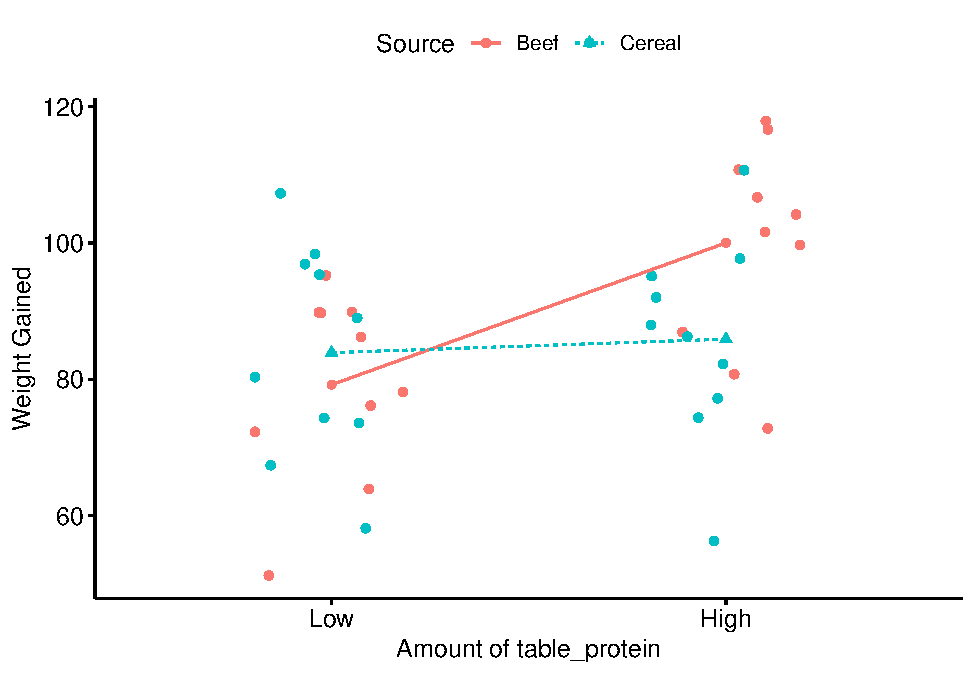
\includegraphics[width=0.3\linewidth]{lab6_stat565_files/figure-latex/unnamed-chunk-3-1}

\begin{enumerate}
\def\labelenumi{(\alph{enumi})}
\setcounter{enumi}{1}
\tightlist
\item
  \textcolor[rgb]{0.5,0.5,0.5}{Obtain the numerical summary for each treatment combination and factor levels separately. Report them here in a tabular form}
\end{enumerate}

\begin{longtable}[]{@{}cccccccccc@{}}
\toprule
\begin{minipage}[b]{0.09\columnwidth}\centering
method\strut
\end{minipage} & \begin{minipage}[b]{0.06\columnwidth}\centering
min\strut
\end{minipage} & \begin{minipage}[b]{0.08\columnwidth}\centering
Q1\strut
\end{minipage} & \begin{minipage}[b]{0.09\columnwidth}\centering
median\strut
\end{minipage} & \begin{minipage}[b]{0.08\columnwidth}\centering
Q3\strut
\end{minipage} & \begin{minipage}[b]{0.06\columnwidth}\centering
max\strut
\end{minipage} & \begin{minipage}[b]{0.08\columnwidth}\centering
mean\strut
\end{minipage} & \begin{minipage}[b]{0.08\columnwidth}\centering
sd\strut
\end{minipage} & \begin{minipage}[b]{0.05\columnwidth}\centering
n\strut
\end{minipage} & \begin{minipage}[b]{0.10\columnwidth}\centering
missing\strut
\end{minipage}\tabularnewline
\midrule
\endhead
\begin{minipage}[t]{0.09\columnwidth}\centering
a\strut
\end{minipage} & \begin{minipage}[t]{0.06\columnwidth}\centering
151\strut
\end{minipage} & \begin{minipage}[t]{0.08\columnwidth}\centering
201.5\strut
\end{minipage} & \begin{minipage}[t]{0.09\columnwidth}\centering
226.5\strut
\end{minipage} & \begin{minipage}[t]{0.08\columnwidth}\centering
268\strut
\end{minipage} & \begin{minipage}[t]{0.06\columnwidth}\centering
286\strut
\end{minipage} & \begin{minipage}[t]{0.08\columnwidth}\centering
230.1\strut
\end{minipage} & \begin{minipage}[t]{0.08\columnwidth}\centering
39.86\strut
\end{minipage} & \begin{minipage}[t]{0.05\columnwidth}\centering
30\strut
\end{minipage} & \begin{minipage}[t]{0.10\columnwidth}\centering
0\strut
\end{minipage}\tabularnewline
\begin{minipage}[t]{0.09\columnwidth}\centering
b\strut
\end{minipage} & \begin{minipage}[t]{0.06\columnwidth}\centering
60\strut
\end{minipage} & \begin{minipage}[t]{0.08\columnwidth}\centering
125.2\strut
\end{minipage} & \begin{minipage}[t]{0.09\columnwidth}\centering
160\strut
\end{minipage} & \begin{minipage}[t]{0.08\columnwidth}\centering
186.5\strut
\end{minipage} & \begin{minipage}[t]{0.06\columnwidth}\centering
270\strut
\end{minipage} & \begin{minipage}[t]{0.08\columnwidth}\centering
157\strut
\end{minipage} & \begin{minipage}[t]{0.08\columnwidth}\centering
48.93\strut
\end{minipage} & \begin{minipage}[t]{0.05\columnwidth}\centering
30\strut
\end{minipage} & \begin{minipage}[t]{0.10\columnwidth}\centering
0\strut
\end{minipage}\tabularnewline
\begin{minipage}[t]{0.09\columnwidth}\centering
c\strut
\end{minipage} & \begin{minipage}[t]{0.06\columnwidth}\centering
63\strut
\end{minipage} & \begin{minipage}[t]{0.08\columnwidth}\centering
143.2\strut
\end{minipage} & \begin{minipage}[t]{0.09\columnwidth}\centering
164.5\strut
\end{minipage} & \begin{minipage}[t]{0.08\columnwidth}\centering
200\strut
\end{minipage} & \begin{minipage}[t]{0.06\columnwidth}\centering
255\strut
\end{minipage} & \begin{minipage}[t]{0.08\columnwidth}\centering
166.1\strut
\end{minipage} & \begin{minipage}[t]{0.08\columnwidth}\centering
49.28\strut
\end{minipage} & \begin{minipage}[t]{0.05\columnwidth}\centering
30\strut
\end{minipage} & \begin{minipage}[t]{0.10\columnwidth}\centering
0\strut
\end{minipage}\tabularnewline
\bottomrule
\end{longtable}

\begin{longtable}[]{@{}cccccccccc@{}}
\toprule
\begin{minipage}[b]{0.09\columnwidth}\centering
variety\strut
\end{minipage} & \begin{minipage}[b]{0.06\columnwidth}\centering
min\strut
\end{minipage} & \begin{minipage}[b]{0.08\columnwidth}\centering
Q1\strut
\end{minipage} & \begin{minipage}[b]{0.09\columnwidth}\centering
median\strut
\end{minipage} & \begin{minipage}[b]{0.08\columnwidth}\centering
Q3\strut
\end{minipage} & \begin{minipage}[b]{0.06\columnwidth}\centering
max\strut
\end{minipage} & \begin{minipage}[b]{0.08\columnwidth}\centering
mean\strut
\end{minipage} & \begin{minipage}[b]{0.08\columnwidth}\centering
sd\strut
\end{minipage} & \begin{minipage}[b]{0.05\columnwidth}\centering
n\strut
\end{minipage} & \begin{minipage}[b]{0.09\columnwidth}\centering
missing\strut
\end{minipage}\tabularnewline
\midrule
\endhead
\begin{minipage}[t]{0.09\columnwidth}\centering
a.1\strut
\end{minipage} & \begin{minipage}[t]{0.06\columnwidth}\centering
181\strut
\end{minipage} & \begin{minipage}[t]{0.08\columnwidth}\centering
198.5\strut
\end{minipage} & \begin{minipage}[t]{0.09\columnwidth}\centering
221\strut
\end{minipage} & \begin{minipage}[t]{0.08\columnwidth}\centering
236\strut
\end{minipage} & \begin{minipage}[t]{0.06\columnwidth}\centering
251\strut
\end{minipage} & \begin{minipage}[t]{0.08\columnwidth}\centering
217.7\strut
\end{minipage} & \begin{minipage}[t]{0.08\columnwidth}\centering
27.33\strut
\end{minipage} & \begin{minipage}[t]{0.05\columnwidth}\centering
6\strut
\end{minipage} & \begin{minipage}[t]{0.09\columnwidth}\centering
0\strut
\end{minipage}\tabularnewline
\begin{minipage}[t]{0.09\columnwidth}\centering
b.1\strut
\end{minipage} & \begin{minipage}[t]{0.06\columnwidth}\centering
60\strut
\end{minipage} & \begin{minipage}[t]{0.08\columnwidth}\centering
120\strut
\end{minipage} & \begin{minipage}[t]{0.09\columnwidth}\centering
140\strut
\end{minipage} & \begin{minipage}[t]{0.08\columnwidth}\centering
171.2\strut
\end{minipage} & \begin{minipage}[t]{0.06\columnwidth}\centering
270\strut
\end{minipage} & \begin{minipage}[t]{0.08\columnwidth}\centering
150.8\strut
\end{minipage} & \begin{minipage}[t]{0.08\columnwidth}\centering
70.53\strut
\end{minipage} & \begin{minipage}[t]{0.05\columnwidth}\centering
6\strut
\end{minipage} & \begin{minipage}[t]{0.09\columnwidth}\centering
0\strut
\end{minipage}\tabularnewline
\begin{minipage}[t]{0.09\columnwidth}\centering
c.1\strut
\end{minipage} & \begin{minipage}[t]{0.06\columnwidth}\centering
145\strut
\end{minipage} & \begin{minipage}[t]{0.08\columnwidth}\centering
167.5\strut
\end{minipage} & \begin{minipage}[t]{0.09\columnwidth}\centering
190\strut
\end{minipage} & \begin{minipage}[t]{0.08\columnwidth}\centering
197.5\strut
\end{minipage} & \begin{minipage}[t]{0.06\columnwidth}\centering
220\strut
\end{minipage} & \begin{minipage}[t]{0.08\columnwidth}\centering
184.2\strut
\end{minipage} & \begin{minipage}[t]{0.08\columnwidth}\centering
27.28\strut
\end{minipage} & \begin{minipage}[t]{0.05\columnwidth}\centering
6\strut
\end{minipage} & \begin{minipage}[t]{0.09\columnwidth}\centering
0\strut
\end{minipage}\tabularnewline
\begin{minipage}[t]{0.09\columnwidth}\centering
a.2\strut
\end{minipage} & \begin{minipage}[t]{0.06\columnwidth}\centering
151\strut
\end{minipage} & \begin{minipage}[t]{0.08\columnwidth}\centering
164.8\strut
\end{minipage} & \begin{minipage}[t]{0.09\columnwidth}\centering
226\strut
\end{minipage} & \begin{minipage}[t]{0.08\columnwidth}\centering
264.8\strut
\end{minipage} & \begin{minipage}[t]{0.06\columnwidth}\centering
286\strut
\end{minipage} & \begin{minipage}[t]{0.08\columnwidth}\centering
218.5\strut
\end{minipage} & \begin{minipage}[t]{0.08\columnwidth}\centering
58.89\strut
\end{minipage} & \begin{minipage}[t]{0.05\columnwidth}\centering
6\strut
\end{minipage} & \begin{minipage}[t]{0.09\columnwidth}\centering
0\strut
\end{minipage}\tabularnewline
\begin{minipage}[t]{0.09\columnwidth}\centering
b.2\strut
\end{minipage} & \begin{minipage}[t]{0.06\columnwidth}\centering
104\strut
\end{minipage} & \begin{minipage}[t]{0.08\columnwidth}\centering
127.8\strut
\end{minipage} & \begin{minipage}[t]{0.09\columnwidth}\centering
161.5\strut
\end{minipage} & \begin{minipage}[t]{0.08\columnwidth}\centering
172.8\strut
\end{minipage} & \begin{minipage}[t]{0.06\columnwidth}\centering
194\strut
\end{minipage} & \begin{minipage}[t]{0.08\columnwidth}\centering
152.3\strut
\end{minipage} & \begin{minipage}[t]{0.08\columnwidth}\centering
34.45\strut
\end{minipage} & \begin{minipage}[t]{0.05\columnwidth}\centering
6\strut
\end{minipage} & \begin{minipage}[t]{0.09\columnwidth}\centering
0\strut
\end{minipage}\tabularnewline
\begin{minipage}[t]{0.09\columnwidth}\centering
c.2\strut
\end{minipage} & \begin{minipage}[t]{0.06\columnwidth}\centering
165\strut
\end{minipage} & \begin{minipage}[t]{0.08\columnwidth}\centering
176.2\strut
\end{minipage} & \begin{minipage}[t]{0.09\columnwidth}\centering
190\strut
\end{minipage} & \begin{minipage}[t]{0.08\columnwidth}\centering
215\strut
\end{minipage} & \begin{minipage}[t]{0.06\columnwidth}\centering
255\strut
\end{minipage} & \begin{minipage}[t]{0.08\columnwidth}\centering
199.2\strut
\end{minipage} & \begin{minipage}[t]{0.08\columnwidth}\centering
33.68\strut
\end{minipage} & \begin{minipage}[t]{0.05\columnwidth}\centering
6\strut
\end{minipage} & \begin{minipage}[t]{0.09\columnwidth}\centering
0\strut
\end{minipage}\tabularnewline
\begin{minipage}[t]{0.09\columnwidth}\centering
a.3\strut
\end{minipage} & \begin{minipage}[t]{0.06\columnwidth}\centering
183\strut
\end{minipage} & \begin{minipage}[t]{0.08\columnwidth}\centering
215.5\strut
\end{minipage} & \begin{minipage}[t]{0.09\columnwidth}\centering
225.5\strut
\end{minipage} & \begin{minipage}[t]{0.08\columnwidth}\centering
250.5\strut
\end{minipage} & \begin{minipage}[t]{0.06\columnwidth}\centering
283\strut
\end{minipage} & \begin{minipage}[t]{0.08\columnwidth}\centering
231.3\strut
\end{minipage} & \begin{minipage}[t]{0.08\columnwidth}\centering
35.02\strut
\end{minipage} & \begin{minipage}[t]{0.05\columnwidth}\centering
6\strut
\end{minipage} & \begin{minipage}[t]{0.09\columnwidth}\centering
0\strut
\end{minipage}\tabularnewline
\begin{minipage}[t]{0.09\columnwidth}\centering
b.3\strut
\end{minipage} & \begin{minipage}[t]{0.06\columnwidth}\centering
102\strut
\end{minipage} & \begin{minipage}[t]{0.08\columnwidth}\centering
130.8\strut
\end{minipage} & \begin{minipage}[t]{0.09\columnwidth}\centering
162\strut
\end{minipage} & \begin{minipage}[t]{0.08\columnwidth}\centering
178.2\strut
\end{minipage} & \begin{minipage}[t]{0.06\columnwidth}\centering
197\strut
\end{minipage} & \begin{minipage}[t]{0.08\columnwidth}\centering
154.5\strut
\end{minipage} & \begin{minipage}[t]{0.08\columnwidth}\centering
36.16\strut
\end{minipage} & \begin{minipage}[t]{0.05\columnwidth}\centering
6\strut
\end{minipage} & \begin{minipage}[t]{0.09\columnwidth}\centering
0\strut
\end{minipage}\tabularnewline
\begin{minipage}[t]{0.09\columnwidth}\centering
c.3\strut
\end{minipage} & \begin{minipage}[t]{0.06\columnwidth}\centering
104\strut
\end{minipage} & \begin{minipage}[t]{0.08\columnwidth}\centering
149\strut
\end{minipage} & \begin{minipage}[t]{0.09\columnwidth}\centering
181.5\strut
\end{minipage} & \begin{minipage}[t]{0.08\columnwidth}\centering
210.2\strut
\end{minipage} & \begin{minipage}[t]{0.06\columnwidth}\centering
214\strut
\end{minipage} & \begin{minipage}[t]{0.08\columnwidth}\centering
173.2\strut
\end{minipage} & \begin{minipage}[t]{0.08\columnwidth}\centering
44.09\strut
\end{minipage} & \begin{minipage}[t]{0.05\columnwidth}\centering
6\strut
\end{minipage} & \begin{minipage}[t]{0.09\columnwidth}\centering
0\strut
\end{minipage}\tabularnewline
\begin{minipage}[t]{0.09\columnwidth}\centering
a.4\strut
\end{minipage} & \begin{minipage}[t]{0.06\columnwidth}\centering
198\strut
\end{minipage} & \begin{minipage}[t]{0.08\columnwidth}\centering
268\strut
\end{minipage} & \begin{minipage}[t]{0.09\columnwidth}\centering
268\strut
\end{minipage} & \begin{minipage}[t]{0.08\columnwidth}\centering
271.8\strut
\end{minipage} & \begin{minipage}[t]{0.06\columnwidth}\centering
283\strut
\end{minipage} & \begin{minipage}[t]{0.08\columnwidth}\centering
259.7\strut
\end{minipage} & \begin{minipage}[t]{0.08\columnwidth}\centering
30.77\strut
\end{minipage} & \begin{minipage}[t]{0.05\columnwidth}\centering
6\strut
\end{minipage} & \begin{minipage}[t]{0.09\columnwidth}\centering
0\strut
\end{minipage}\tabularnewline
\begin{minipage}[t]{0.09\columnwidth}\centering
b.4\strut
\end{minipage} & \begin{minipage}[t]{0.06\columnwidth}\centering
65\strut
\end{minipage} & \begin{minipage}[t]{0.08\columnwidth}\centering
91\strut
\end{minipage} & \begin{minipage}[t]{0.09\columnwidth}\centering
143.5\strut
\end{minipage} & \begin{minipage}[t]{0.08\columnwidth}\centering
166\strut
\end{minipage} & \begin{minipage}[t]{0.06\columnwidth}\centering
211\strut
\end{minipage} & \begin{minipage}[t]{0.08\columnwidth}\centering
135\strut
\end{minipage} & \begin{minipage}[t]{0.08\columnwidth}\centering
56.05\strut
\end{minipage} & \begin{minipage}[t]{0.05\columnwidth}\centering
6\strut
\end{minipage} & \begin{minipage}[t]{0.09\columnwidth}\centering
0\strut
\end{minipage}\tabularnewline
\begin{minipage}[t]{0.09\columnwidth}\centering
c.4\strut
\end{minipage} & \begin{minipage}[t]{0.06\columnwidth}\centering
75\strut
\end{minipage} & \begin{minipage}[t]{0.08\columnwidth}\centering
118.8\strut
\end{minipage} & \begin{minipage}[t]{0.09\columnwidth}\centering
150\strut
\end{minipage} & \begin{minipage}[t]{0.08\columnwidth}\centering
158.8\strut
\end{minipage} & \begin{minipage}[t]{0.06\columnwidth}\centering
245\strut
\end{minipage} & \begin{minipage}[t]{0.08\columnwidth}\centering
148.3\strut
\end{minipage} & \begin{minipage}[t]{0.08\columnwidth}\centering
57.24\strut
\end{minipage} & \begin{minipage}[t]{0.05\columnwidth}\centering
6\strut
\end{minipage} & \begin{minipage}[t]{0.09\columnwidth}\centering
0\strut
\end{minipage}\tabularnewline
\begin{minipage}[t]{0.09\columnwidth}\centering
a.5\strut
\end{minipage} & \begin{minipage}[t]{0.06\columnwidth}\centering
170\strut
\end{minipage} & \begin{minipage}[t]{0.08\columnwidth}\centering
206.2\strut
\end{minipage} & \begin{minipage}[t]{0.09\columnwidth}\centering
225\strut
\end{minipage} & \begin{minipage}[t]{0.08\columnwidth}\centering
236.2\strut
\end{minipage} & \begin{minipage}[t]{0.06\columnwidth}\centering
280\strut
\end{minipage} & \begin{minipage}[t]{0.08\columnwidth}\centering
223.3\strut
\end{minipage} & \begin{minipage}[t]{0.08\columnwidth}\centering
37.1\strut
\end{minipage} & \begin{minipage}[t]{0.05\columnwidth}\centering
6\strut
\end{minipage} & \begin{minipage}[t]{0.09\columnwidth}\centering
0\strut
\end{minipage}\tabularnewline
\begin{minipage}[t]{0.09\columnwidth}\centering
b.5\strut
\end{minipage} & \begin{minipage}[t]{0.06\columnwidth}\centering
143\strut
\end{minipage} & \begin{minipage}[t]{0.08\columnwidth}\centering
169.2\strut
\end{minipage} & \begin{minipage}[t]{0.09\columnwidth}\centering
200.5\strut
\end{minipage} & \begin{minipage}[t]{0.08\columnwidth}\centering
216.8\strut
\end{minipage} & \begin{minipage}[t]{0.06\columnwidth}\centering
228\strut
\end{minipage} & \begin{minipage}[t]{0.08\columnwidth}\centering
192.2\strut
\end{minipage} & \begin{minipage}[t]{0.08\columnwidth}\centering
33.68\strut
\end{minipage} & \begin{minipage}[t]{0.05\columnwidth}\centering
6\strut
\end{minipage} & \begin{minipage}[t]{0.09\columnwidth}\centering
0\strut
\end{minipage}\tabularnewline
\begin{minipage}[t]{0.09\columnwidth}\centering
c.5\strut
\end{minipage} & \begin{minipage}[t]{0.06\columnwidth}\centering
63\strut
\end{minipage} & \begin{minipage}[t]{0.08\columnwidth}\centering
88\strut
\end{minipage} & \begin{minipage}[t]{0.09\columnwidth}\centering
128\strut
\end{minipage} & \begin{minipage}[t]{0.08\columnwidth}\centering
141.8\strut
\end{minipage} & \begin{minipage}[t]{0.06\columnwidth}\centering
213\strut
\end{minipage} & \begin{minipage}[t]{0.08\columnwidth}\centering
125.5\strut
\end{minipage} & \begin{minipage}[t]{0.08\columnwidth}\centering
53.55\strut
\end{minipage} & \begin{minipage}[t]{0.05\columnwidth}\centering
6\strut
\end{minipage} & \begin{minipage}[t]{0.09\columnwidth}\centering
0\strut
\end{minipage}\tabularnewline
\begin{minipage}[t]{0.09\columnwidth}\centering
1\strut
\end{minipage} & \begin{minipage}[t]{0.06\columnwidth}\centering
60\strut
\end{minipage} & \begin{minipage}[t]{0.08\columnwidth}\centering
148.8\strut
\end{minipage} & \begin{minipage}[t]{0.09\columnwidth}\centering
190\strut
\end{minipage} & \begin{minipage}[t]{0.08\columnwidth}\centering
220.8\strut
\end{minipage} & \begin{minipage}[t]{0.06\columnwidth}\centering
270\strut
\end{minipage} & \begin{minipage}[t]{0.08\columnwidth}\centering
184.2\strut
\end{minipage} & \begin{minipage}[t]{0.08\columnwidth}\centering
51.86\strut
\end{minipage} & \begin{minipage}[t]{0.05\columnwidth}\centering
18\strut
\end{minipage} & \begin{minipage}[t]{0.09\columnwidth}\centering
0\strut
\end{minipage}\tabularnewline
\begin{minipage}[t]{0.09\columnwidth}\centering
2\strut
\end{minipage} & \begin{minipage}[t]{0.06\columnwidth}\centering
104\strut
\end{minipage} & \begin{minipage}[t]{0.08\columnwidth}\centering
156.8\strut
\end{minipage} & \begin{minipage}[t]{0.09\columnwidth}\centering
177.5\strut
\end{minipage} & \begin{minipage}[t]{0.08\columnwidth}\centering
216.5\strut
\end{minipage} & \begin{minipage}[t]{0.06\columnwidth}\centering
286\strut
\end{minipage} & \begin{minipage}[t]{0.08\columnwidth}\centering
190\strut
\end{minipage} & \begin{minipage}[t]{0.08\columnwidth}\centering
50.19\strut
\end{minipage} & \begin{minipage}[t]{0.05\columnwidth}\centering
18\strut
\end{minipage} & \begin{minipage}[t]{0.09\columnwidth}\centering
0\strut
\end{minipage}\tabularnewline
\begin{minipage}[t]{0.09\columnwidth}\centering
3\strut
\end{minipage} & \begin{minipage}[t]{0.06\columnwidth}\centering
102\strut
\end{minipage} & \begin{minipage}[t]{0.08\columnwidth}\centering
158.8\strut
\end{minipage} & \begin{minipage}[t]{0.09\columnwidth}\centering
190\strut
\end{minipage} & \begin{minipage}[t]{0.08\columnwidth}\centering
214\strut
\end{minipage} & \begin{minipage}[t]{0.06\columnwidth}\centering
283\strut
\end{minipage} & \begin{minipage}[t]{0.08\columnwidth}\centering
186.3\strut
\end{minipage} & \begin{minipage}[t]{0.08\columnwidth}\centering
49.5\strut
\end{minipage} & \begin{minipage}[t]{0.05\columnwidth}\centering
18\strut
\end{minipage} & \begin{minipage}[t]{0.09\columnwidth}\centering
0\strut
\end{minipage}\tabularnewline
\begin{minipage}[t]{0.09\columnwidth}\centering
4\strut
\end{minipage} & \begin{minipage}[t]{0.06\columnwidth}\centering
65\strut
\end{minipage} & \begin{minipage}[t]{0.08\columnwidth}\centering
138.2\strut
\end{minipage} & \begin{minipage}[t]{0.09\columnwidth}\centering
165.5\strut
\end{minipage} & \begin{minipage}[t]{0.08\columnwidth}\centering
262.2\strut
\end{minipage} & \begin{minipage}[t]{0.06\columnwidth}\centering
283\strut
\end{minipage} & \begin{minipage}[t]{0.08\columnwidth}\centering
181\strut
\end{minipage} & \begin{minipage}[t]{0.08\columnwidth}\centering
73.99\strut
\end{minipage} & \begin{minipage}[t]{0.05\columnwidth}\centering
18\strut
\end{minipage} & \begin{minipage}[t]{0.09\columnwidth}\centering
0\strut
\end{minipage}\tabularnewline
\begin{minipage}[t]{0.09\columnwidth}\centering
5\strut
\end{minipage} & \begin{minipage}[t]{0.06\columnwidth}\centering
63\strut
\end{minipage} & \begin{minipage}[t]{0.08\columnwidth}\centering
143\strut
\end{minipage} & \begin{minipage}[t]{0.09\columnwidth}\centering
194\strut
\end{minipage} & \begin{minipage}[t]{0.08\columnwidth}\centering
223.2\strut
\end{minipage} & \begin{minipage}[t]{0.06\columnwidth}\centering
280\strut
\end{minipage} & \begin{minipage}[t]{0.08\columnwidth}\centering
180.3\strut
\end{minipage} & \begin{minipage}[t]{0.08\columnwidth}\centering
57.84\strut
\end{minipage} & \begin{minipage}[t]{0.05\columnwidth}\centering
18\strut
\end{minipage} & \begin{minipage}[t]{0.09\columnwidth}\centering
0\strut
\end{minipage}\tabularnewline
\bottomrule
\end{longtable}

\begin{enumerate}
\def\labelenumi{(\alph{enumi})}
\setcounter{enumi}{2}
\tightlist
\item
  \textcolor[rgb]{0.5,0.5,0.5}{Fit the two-factor factorial model and report the complete ANOVA table here. Do not report code here. The complete ANOVA table should have a row for each of the following: main effects of each treatment, two-factor interaction effects, error and total}
\end{enumerate}

\begin{longtable}[]{@{}cllllc@{}}
\toprule
\begin{minipage}[b]{0.19\columnwidth}\centering
~\strut
\end{minipage} & \begin{minipage}[b]{0.06\columnwidth}\raggedright
Df\strut
\end{minipage} & \begin{minipage}[b]{0.10\columnwidth}\raggedright
Sum Sq\strut
\end{minipage} & \begin{minipage}[b]{0.12\columnwidth}\raggedright
Mean Sq\strut
\end{minipage} & \begin{minipage}[b]{0.12\columnwidth}\raggedright
F value\strut
\end{minipage} & \begin{minipage}[b]{0.14\columnwidth}\centering
Pr(\textgreater{}F)\strut
\end{minipage}\tabularnewline
\midrule
\endhead
\begin{minipage}[t]{0.19\columnwidth}\centering
\textbf{m}\strut
\end{minipage} & \begin{minipage}[t]{0.06\columnwidth}\raggedright
2\strut
\end{minipage} & \begin{minipage}[t]{0.10\columnwidth}\raggedright
95316\strut
\end{minipage} & \begin{minipage}[t]{0.12\columnwidth}\raggedright
47658\strut
\end{minipage} & \begin{minipage}[t]{0.12\columnwidth}\raggedright
24.25\strut
\end{minipage} & \begin{minipage}[t]{0.14\columnwidth}\centering
7.525e-09\strut
\end{minipage}\tabularnewline
\begin{minipage}[t]{0.19\columnwidth}\centering
\textbf{v}\strut
\end{minipage} & \begin{minipage}[t]{0.06\columnwidth}\raggedright
4\strut
\end{minipage} & \begin{minipage}[t]{0.10\columnwidth}\raggedright
1138\strut
\end{minipage} & \begin{minipage}[t]{0.12\columnwidth}\raggedright
284.5\strut
\end{minipage} & \begin{minipage}[t]{0.12\columnwidth}\raggedright
0.1448\strut
\end{minipage} & \begin{minipage}[t]{0.14\columnwidth}\centering
0.9648\strut
\end{minipage}\tabularnewline
\begin{minipage}[t]{0.19\columnwidth}\centering
\textbf{m:v}\strut
\end{minipage} & \begin{minipage}[t]{0.06\columnwidth}\raggedright
8\strut
\end{minipage} & \begin{minipage}[t]{0.10\columnwidth}\raggedright
37449\strut
\end{minipage} & \begin{minipage}[t]{0.12\columnwidth}\raggedright
4681\strut
\end{minipage} & \begin{minipage}[t]{0.12\columnwidth}\raggedright
2.382\strut
\end{minipage} & \begin{minipage}[t]{0.14\columnwidth}\centering
0.02409\strut
\end{minipage}\tabularnewline
\begin{minipage}[t]{0.19\columnwidth}\centering
\textbf{Residuals}\strut
\end{minipage} & \begin{minipage}[t]{0.06\columnwidth}\raggedright
75\strut
\end{minipage} & \begin{minipage}[t]{0.10\columnwidth}\raggedright
147377\strut
\end{minipage} & \begin{minipage}[t]{0.12\columnwidth}\raggedright
1965\strut
\end{minipage} & \begin{minipage}[t]{0.12\columnwidth}\raggedright
NA\strut
\end{minipage} & \begin{minipage}[t]{0.14\columnwidth}\centering
NA\strut
\end{minipage}\tabularnewline
\begin{minipage}[t]{0.19\columnwidth}\centering
\textbf{Total}\strut
\end{minipage} & \begin{minipage}[t]{0.06\columnwidth}\raggedright
89\strut
\end{minipage} & \begin{minipage}[t]{0.10\columnwidth}\raggedright
281279.2\strut
\end{minipage} & \begin{minipage}[t]{0.12\columnwidth}\raggedright
3160.44\strut
\end{minipage} & \begin{minipage}[t]{0.12\columnwidth}\raggedright
NA\strut
\end{minipage} & \begin{minipage}[t]{0.14\columnwidth}\centering
NA\strut
\end{minipage}\tabularnewline
\bottomrule
\end{longtable}

\begin{enumerate}
\def\labelenumi{(\alph{enumi})}
\setcounter{enumi}{3}
\tightlist
\item
  \textcolor[rgb]{0.5,0.5,0.5}{Based on the ANOVA table write your conclusion appropriately. Perform all the necessary tests and report the conclusion along with the p-value.}
\end{enumerate}

The line plot shows that not all lines are parallel. Difference in y
between methods is not same for different varieties. There could be an
interaction effect.

According to ANOVA table, there is a significant interaction effect from
methods and varieties on the y at 5\% significance level
(P-value=0.02409). That means, effect of method and effect of methods
and varieties on y is not independent. Therefore, examie the simple
effects.

The table shows the multiple comparisons of levels in varieties and
methods.

The difference in y between varieties 2 and 5 is significant when method
c is applies (P-value=0.0295).

The difference in y between method a and b are significant when
varieties 1 - 4 is applies (P-value=0.0290, 0.0310, 0.0101,
\textless{}.0001, respectively).

The difference in y between method a and c are significant when
varieties 4, 5 is applies (P-value=0.0001, 0.0008, respectively).

The difference in y between method b and c is significant when varieties
5 is applies (P-value=0.0295).

The Tukey test indicates the difference in y between method a and b, a
and c are significant when varieties 4 is applies (P-value=0.0002,
0.0015, respectively), the difference in y between method a and c is
significant when varieties 5 is applies (P-value=0.0096).

The difference in y between varieties 1-5 applied method a and varieties
5 applied method c are significant (P-value=0.0383, 0.0349, 0.0074,
0.0001, 0.0199, respectively).

The difference in y between varieties 1-4 applied method b and varieties
4 applied method a are significant (P-value=0.0050, 0.0061, 0.0080,
0.0006, respectively).

The difference in y between varieties 4 applied method b and varieties 3
applied method a are significant (P-value=0.0238).

The Scheffe methods indicates the difference in y between varieties 4
applied method a and varieties 5 applied method c are significant
(P-value=0.0326).

\begin{longtable}[]{@{}crcrlll@{}}
\toprule
\begin{minipage}[b]{0.16\columnwidth}\centering
contrast\strut
\end{minipage} & \begin{minipage}[b]{0.11\columnwidth}\raggedleft
estimate\strut
\end{minipage} & \begin{minipage}[b]{0.07\columnwidth}\centering
SE\strut
\end{minipage} & \begin{minipage}[b]{0.04\columnwidth}\raggedleft
df\strut
\end{minipage} & \begin{minipage}[b]{0.09\columnwidth}\raggedright
t.ratio\strut
\end{minipage} & \begin{minipage}[b]{0.09\columnwidth}\raggedright
p.value\strut
\end{minipage} & \begin{minipage}[b]{0.13\columnwidth}\raggedright
P.adj\strut
\end{minipage}\tabularnewline
\midrule
\endhead
\begin{minipage}[t]{0.16\columnwidth}\centering
c: v2-v5\strut
\end{minipage} & \begin{minipage}[t]{0.11\columnwidth}\raggedleft
73.667\strut
\end{minipage} & \begin{minipage}[t]{0.07\columnwidth}\centering
25.6\strut
\end{minipage} & \begin{minipage}[t]{0.04\columnwidth}\raggedleft
75\strut
\end{minipage} & \begin{minipage}[t]{0.09\columnwidth}\raggedright
2.878\strut
\end{minipage} & \begin{minipage}[t]{0.09\columnwidth}\raggedright
0.0404\strut
\end{minipage} & \begin{minipage}[t]{0.13\columnwidth}\raggedright
\strut
\end{minipage}\tabularnewline
\begin{minipage}[t]{0.16\columnwidth}\centering
v1: a-b\strut
\end{minipage} & \begin{minipage}[t]{0.11\columnwidth}\raggedleft
66.8\strut
\end{minipage} & \begin{minipage}[t]{0.07\columnwidth}\centering
25.6\strut
\end{minipage} & \begin{minipage}[t]{0.04\columnwidth}\raggedleft
75\strut
\end{minipage} & \begin{minipage}[t]{0.09\columnwidth}\raggedright
2.611\strut
\end{minipage} & \begin{minipage}[t]{0.09\columnwidth}\raggedright
0.0290\strut
\end{minipage} & \begin{minipage}[t]{0.13\columnwidth}\raggedright
\strut
\end{minipage}\tabularnewline
\begin{minipage}[t]{0.16\columnwidth}\centering
v2: a-b\strut
\end{minipage} & \begin{minipage}[t]{0.11\columnwidth}\raggedleft
66.2\strut
\end{minipage} & \begin{minipage}[t]{0.07\columnwidth}\centering
25.6\strut
\end{minipage} & \begin{minipage}[t]{0.04\columnwidth}\raggedleft
75\strut
\end{minipage} & \begin{minipage}[t]{0.09\columnwidth}\raggedright
2.585\strut
\end{minipage} & \begin{minipage}[t]{0.09\columnwidth}\raggedright
0.0310\strut
\end{minipage} & \begin{minipage}[t]{0.13\columnwidth}\raggedright
\strut
\end{minipage}\tabularnewline
\begin{minipage}[t]{0.16\columnwidth}\centering
v3: a-b\strut
\end{minipage} & \begin{minipage}[t]{0.11\columnwidth}\raggedleft
76.8\strut
\end{minipage} & \begin{minipage}[t]{0.07\columnwidth}\centering
25.6\strut
\end{minipage} & \begin{minipage}[t]{0.04\columnwidth}\raggedleft
75\strut
\end{minipage} & \begin{minipage}[t]{0.09\columnwidth}\raggedright
3.002\strut
\end{minipage} & \begin{minipage}[t]{0.09\columnwidth}\raggedright
0.0101\strut
\end{minipage} & \begin{minipage}[t]{0.13\columnwidth}\raggedright
Tukey\strut
\end{minipage}\tabularnewline
\begin{minipage}[t]{0.16\columnwidth}\centering
v4: a-b\strut
\end{minipage} & \begin{minipage}[t]{0.11\columnwidth}\raggedleft
124.7\strut
\end{minipage} & \begin{minipage}[t]{0.07\columnwidth}\centering
25.6\strut
\end{minipage} & \begin{minipage}[t]{0.04\columnwidth}\raggedleft
75\strut
\end{minipage} & \begin{minipage}[t]{0.09\columnwidth}\raggedright
4.871\strut
\end{minipage} & \begin{minipage}[t]{0.09\columnwidth}\raggedright
\textless{}.0001\strut
\end{minipage} & \begin{minipage}[t]{0.13\columnwidth}\raggedright
0.0002\strut
\end{minipage}\tabularnewline
\begin{minipage}[t]{0.16\columnwidth}\centering
v4: a-c\strut
\end{minipage} & \begin{minipage}[t]{0.11\columnwidth}\raggedleft
111.3\strut
\end{minipage} & \begin{minipage}[t]{0.07\columnwidth}\centering
25.6\strut
\end{minipage} & \begin{minipage}[t]{0.04\columnwidth}\raggedleft
75\strut
\end{minipage} & \begin{minipage}[t]{0.09\columnwidth}\raggedright
4.350\strut
\end{minipage} & \begin{minipage}[t]{0.09\columnwidth}\raggedright
0.0001\strut
\end{minipage} & \begin{minipage}[t]{0.13\columnwidth}\raggedright
0.0016\strut
\end{minipage}\tabularnewline
\begin{minipage}[t]{0.16\columnwidth}\centering
v5: a-c\strut
\end{minipage} & \begin{minipage}[t]{0.11\columnwidth}\raggedleft
97.8\strut
\end{minipage} & \begin{minipage}[t]{0.07\columnwidth}\centering
25.6\strut
\end{minipage} & \begin{minipage}[t]{0.04\columnwidth}\raggedleft
75\strut
\end{minipage} & \begin{minipage}[t]{0.09\columnwidth}\raggedright
3.823\strut
\end{minipage} & \begin{minipage}[t]{0.09\columnwidth}\raggedright
0.0008\strut
\end{minipage} & \begin{minipage}[t]{0.13\columnwidth}\raggedright
0.0096\strut
\end{minipage}\tabularnewline
\begin{minipage}[t]{0.16\columnwidth}\centering
v5: b-c\strut
\end{minipage} & \begin{minipage}[t]{0.11\columnwidth}\raggedleft
66.7\strut
\end{minipage} & \begin{minipage}[t]{0.07\columnwidth}\centering
25.6\strut
\end{minipage} & \begin{minipage}[t]{0.04\columnwidth}\raggedleft
75\strut
\end{minipage} & \begin{minipage}[t]{0.09\columnwidth}\raggedright
2.605\strut
\end{minipage} & \begin{minipage}[t]{0.09\columnwidth}\raggedright
0.0295\strut
\end{minipage} & \begin{minipage}[t]{0.13\columnwidth}\raggedright
\strut
\end{minipage}\tabularnewline
\begin{minipage}[t]{0.16\columnwidth}\centering
\strut
\end{minipage} & \begin{minipage}[t]{0.11\columnwidth}\raggedleft
\strut
\end{minipage} & \begin{minipage}[t]{0.07\columnwidth}\centering
\strut
\end{minipage} & \begin{minipage}[t]{0.04\columnwidth}\raggedleft
\strut
\end{minipage} & \begin{minipage}[t]{0.09\columnwidth}\raggedright
\strut
\end{minipage} & \begin{minipage}[t]{0.09\columnwidth}\raggedright
\strut
\end{minipage} & \begin{minipage}[t]{0.13\columnwidth}\raggedright
\strut
\end{minipage}\tabularnewline
\begin{minipage}[t]{0.16\columnwidth}\centering
v1,a-v5,c\strut
\end{minipage} & \begin{minipage}[t]{0.11\columnwidth}\raggedleft
92.167\strut
\end{minipage} & \begin{minipage}[t]{0.07\columnwidth}\centering
25.6\strut
\end{minipage} & \begin{minipage}[t]{0.04\columnwidth}\raggedleft
75\strut
\end{minipage} & \begin{minipage}[t]{0.09\columnwidth}\raggedright
3.601\strut
\end{minipage} & \begin{minipage}[t]{0.09\columnwidth}\raggedright
0.0383\strut
\end{minipage} & \begin{minipage}[t]{0.13\columnwidth}\raggedright
\strut
\end{minipage}\tabularnewline
\begin{minipage}[t]{0.16\columnwidth}\centering
v2,a-v5,c\strut
\end{minipage} & \begin{minipage}[t]{0.11\columnwidth}\raggedleft
93.000\strut
\end{minipage} & \begin{minipage}[t]{0.07\columnwidth}\centering
25.6\strut
\end{minipage} & \begin{minipage}[t]{0.04\columnwidth}\raggedleft
75\strut
\end{minipage} & \begin{minipage}[t]{0.09\columnwidth}\raggedright
3.634\strut
\end{minipage} & \begin{minipage}[t]{0.09\columnwidth}\raggedright
0.0349\strut
\end{minipage} & \begin{minipage}[t]{0.13\columnwidth}\raggedright
\strut
\end{minipage}\tabularnewline
\begin{minipage}[t]{0.16\columnwidth}\centering
v3,a-v4,b\strut
\end{minipage} & \begin{minipage}[t]{0.11\columnwidth}\raggedleft
96.333\strut
\end{minipage} & \begin{minipage}[t]{0.07\columnwidth}\centering
25.6\strut
\end{minipage} & \begin{minipage}[t]{0.04\columnwidth}\raggedleft
75\strut
\end{minipage} & \begin{minipage}[t]{0.09\columnwidth}\raggedright
3.764\strut
\end{minipage} & \begin{minipage}[t]{0.09\columnwidth}\raggedright
0.0238\strut
\end{minipage} & \begin{minipage}[t]{0.13\columnwidth}\raggedright
\strut
\end{minipage}\tabularnewline
\begin{minipage}[t]{0.16\columnwidth}\centering
v3,a-v5,c\strut
\end{minipage} & \begin{minipage}[t]{0.11\columnwidth}\raggedleft
105.833\strut
\end{minipage} & \begin{minipage}[t]{0.07\columnwidth}\centering
25.6\strut
\end{minipage} & \begin{minipage}[t]{0.04\columnwidth}\raggedleft
75\strut
\end{minipage} & \begin{minipage}[t]{0.09\columnwidth}\raggedright
4.135\strut
\end{minipage} & \begin{minipage}[t]{0.09\columnwidth}\raggedright
0.0074\strut
\end{minipage} & \begin{minipage}[t]{0.13\columnwidth}\raggedright
\strut
\end{minipage}\tabularnewline
\begin{minipage}[t]{0.16\columnwidth}\centering
v4,a-v1,b\strut
\end{minipage} & \begin{minipage}[t]{0.11\columnwidth}\raggedleft
108.833\strut
\end{minipage} & \begin{minipage}[t]{0.07\columnwidth}\centering
25.6\strut
\end{minipage} & \begin{minipage}[t]{0.04\columnwidth}\raggedleft
75\strut
\end{minipage} & \begin{minipage}[t]{0.09\columnwidth}\raggedright
4.252\strut
\end{minipage} & \begin{minipage}[t]{0.09\columnwidth}\raggedright
0.0050\strut
\end{minipage} & \begin{minipage}[t]{0.13\columnwidth}\raggedright
\strut
\end{minipage}\tabularnewline
\begin{minipage}[t]{0.16\columnwidth}\centering
v4,a-v2,b\strut
\end{minipage} & \begin{minipage}[t]{0.11\columnwidth}\raggedleft
107.333\strut
\end{minipage} & \begin{minipage}[t]{0.07\columnwidth}\centering
25.6\strut
\end{minipage} & \begin{minipage}[t]{0.04\columnwidth}\raggedleft
75\strut
\end{minipage} & \begin{minipage}[t]{0.09\columnwidth}\raggedright
4.194\strut
\end{minipage} & \begin{minipage}[t]{0.09\columnwidth}\raggedright
0.0061\strut
\end{minipage} & \begin{minipage}[t]{0.13\columnwidth}\raggedright
\strut
\end{minipage}\tabularnewline
\begin{minipage}[t]{0.16\columnwidth}\centering
v4,a-v3,b\strut
\end{minipage} & \begin{minipage}[t]{0.11\columnwidth}\raggedleft
105.167\strut
\end{minipage} & \begin{minipage}[t]{0.07\columnwidth}\centering
25.6\strut
\end{minipage} & \begin{minipage}[t]{0.04\columnwidth}\raggedleft
75\strut
\end{minipage} & \begin{minipage}[t]{0.09\columnwidth}\raggedright
4.109\strut
\end{minipage} & \begin{minipage}[t]{0.09\columnwidth}\raggedright
0.0080\strut
\end{minipage} & \begin{minipage}[t]{0.13\columnwidth}\raggedright
\strut
\end{minipage}\tabularnewline
\begin{minipage}[t]{0.16\columnwidth}\centering
v4,a-v4,b\strut
\end{minipage} & \begin{minipage}[t]{0.11\columnwidth}\raggedleft
124.667\strut
\end{minipage} & \begin{minipage}[t]{0.07\columnwidth}\centering
25.6\strut
\end{minipage} & \begin{minipage}[t]{0.04\columnwidth}\raggedleft
75\strut
\end{minipage} & \begin{minipage}[t]{0.09\columnwidth}\raggedright
4.871\strut
\end{minipage} & \begin{minipage}[t]{0.09\columnwidth}\raggedright
0.0006\strut
\end{minipage} & \begin{minipage}[t]{0.13\columnwidth}\raggedright
\strut
\end{minipage}\tabularnewline
\begin{minipage}[t]{0.16\columnwidth}\centering
v4,a-v4,c\strut
\end{minipage} & \begin{minipage}[t]{0.11\columnwidth}\raggedleft
111.333\strut
\end{minipage} & \begin{minipage}[t]{0.07\columnwidth}\centering
25.6\strut
\end{minipage} & \begin{minipage}[t]{0.04\columnwidth}\raggedleft
75\strut
\end{minipage} & \begin{minipage}[t]{0.09\columnwidth}\raggedright
4.350\strut
\end{minipage} & \begin{minipage}[t]{0.09\columnwidth}\raggedright
0.0036\strut
\end{minipage} & \begin{minipage}[t]{0.13\columnwidth}\raggedright
Scheffe\strut
\end{minipage}\tabularnewline
\begin{minipage}[t]{0.16\columnwidth}\centering
v4,a-v5,c\strut
\end{minipage} & \begin{minipage}[t]{0.11\columnwidth}\raggedleft
134.167\strut
\end{minipage} & \begin{minipage}[t]{0.07\columnwidth}\centering
25.6\strut
\end{minipage} & \begin{minipage}[t]{0.04\columnwidth}\raggedleft
75\strut
\end{minipage} & \begin{minipage}[t]{0.09\columnwidth}\raggedright
5.242\strut
\end{minipage} & \begin{minipage}[t]{0.09\columnwidth}\raggedright
0.0001\strut
\end{minipage} & \begin{minipage}[t]{0.13\columnwidth}\raggedright
0.0326\strut
\end{minipage}\tabularnewline
\begin{minipage}[t]{0.16\columnwidth}\centering
v5,a-v5,c\strut
\end{minipage} & \begin{minipage}[t]{0.11\columnwidth}\raggedleft
97.833\strut
\end{minipage} & \begin{minipage}[t]{0.07\columnwidth}\centering
25.6\strut
\end{minipage} & \begin{minipage}[t]{0.04\columnwidth}\raggedleft
75\strut
\end{minipage} & \begin{minipage}[t]{0.09\columnwidth}\raggedright
3.823\strut
\end{minipage} & \begin{minipage}[t]{0.09\columnwidth}\raggedright
0.0199\strut
\end{minipage} & \begin{minipage}[t]{0.13\columnwidth}\raggedright
\strut
\end{minipage}\tabularnewline
\bottomrule
\end{longtable}

\begin{enumerate}
\def\labelenumi{(\alph{enumi})}
\setcounter{enumi}{4}
\tightlist
\item
  \textcolor[rgb]{0.5,0.5,0.5}{Provide the plots of residuals here. Do not report code here.}
\end{enumerate}

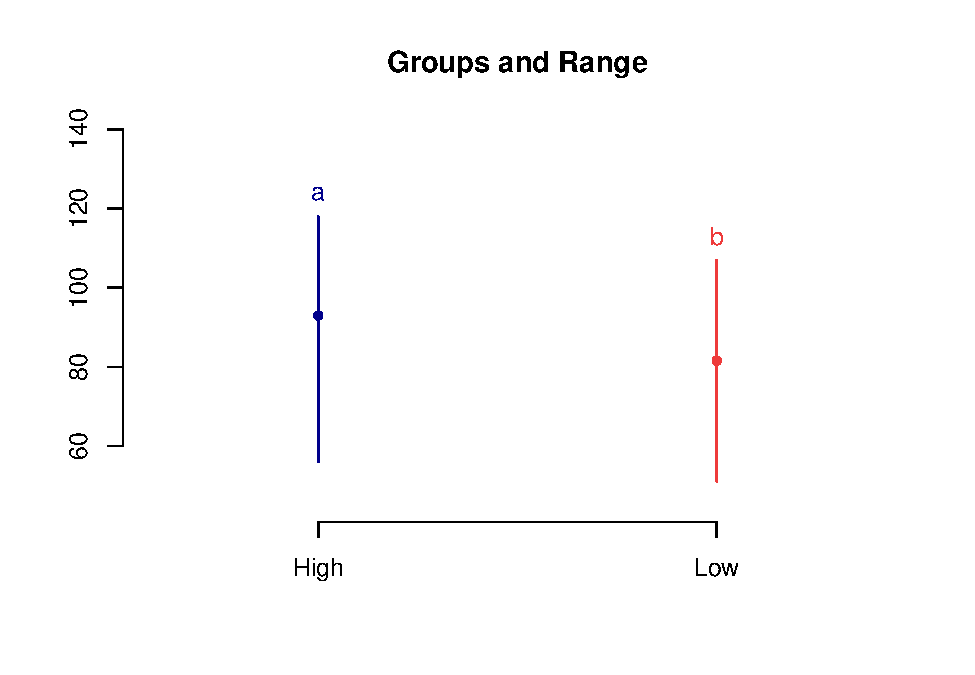
\includegraphics[width=0.25\linewidth]{lab6_stat565_files/figure-latex/unnamed-chunk-6-1}
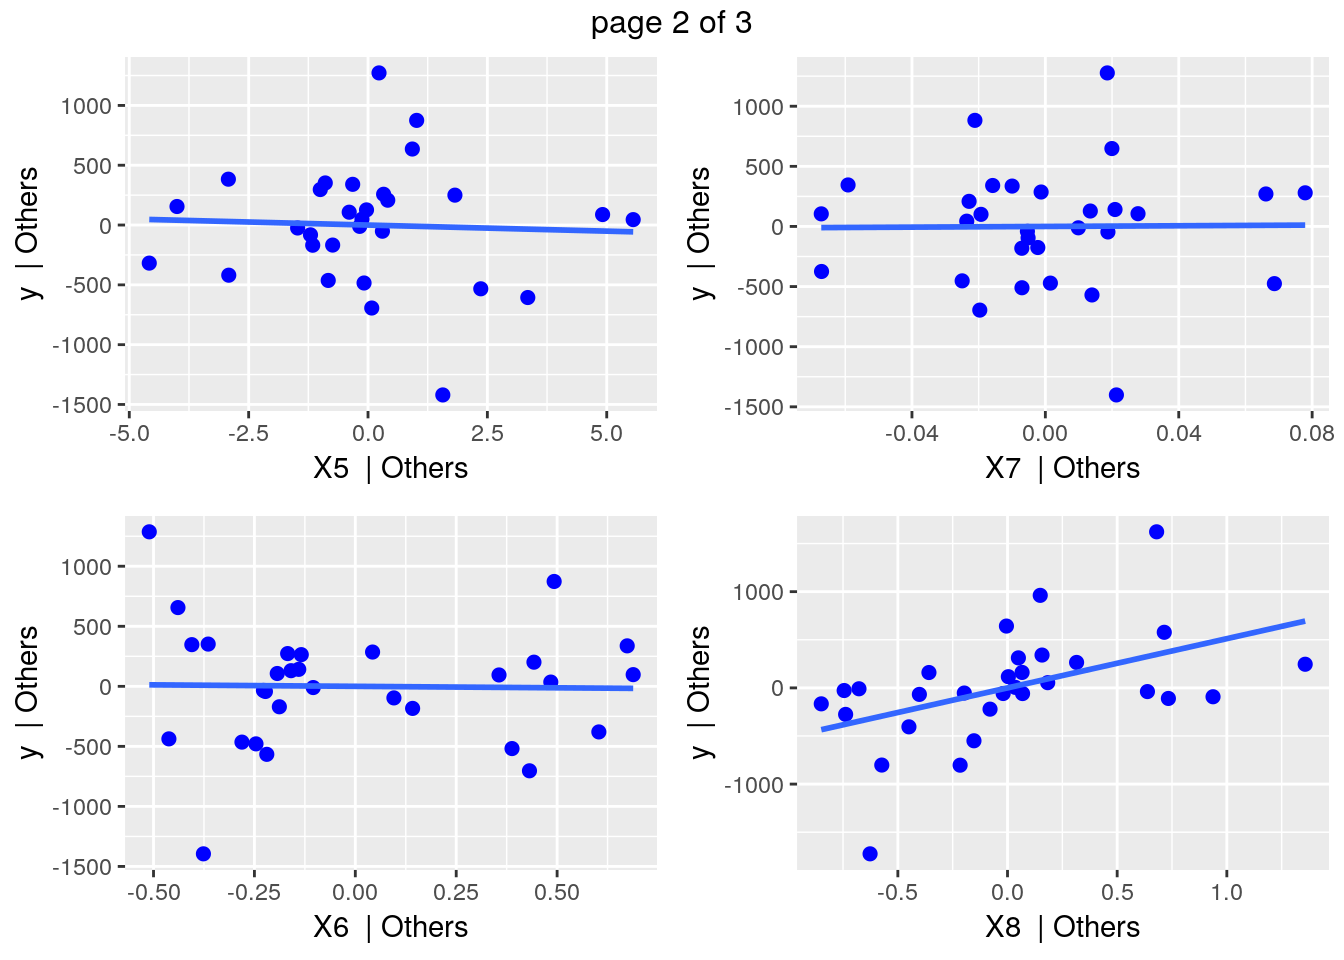
\includegraphics[width=0.25\linewidth]{lab6_stat565_files/figure-latex/unnamed-chunk-6-2}
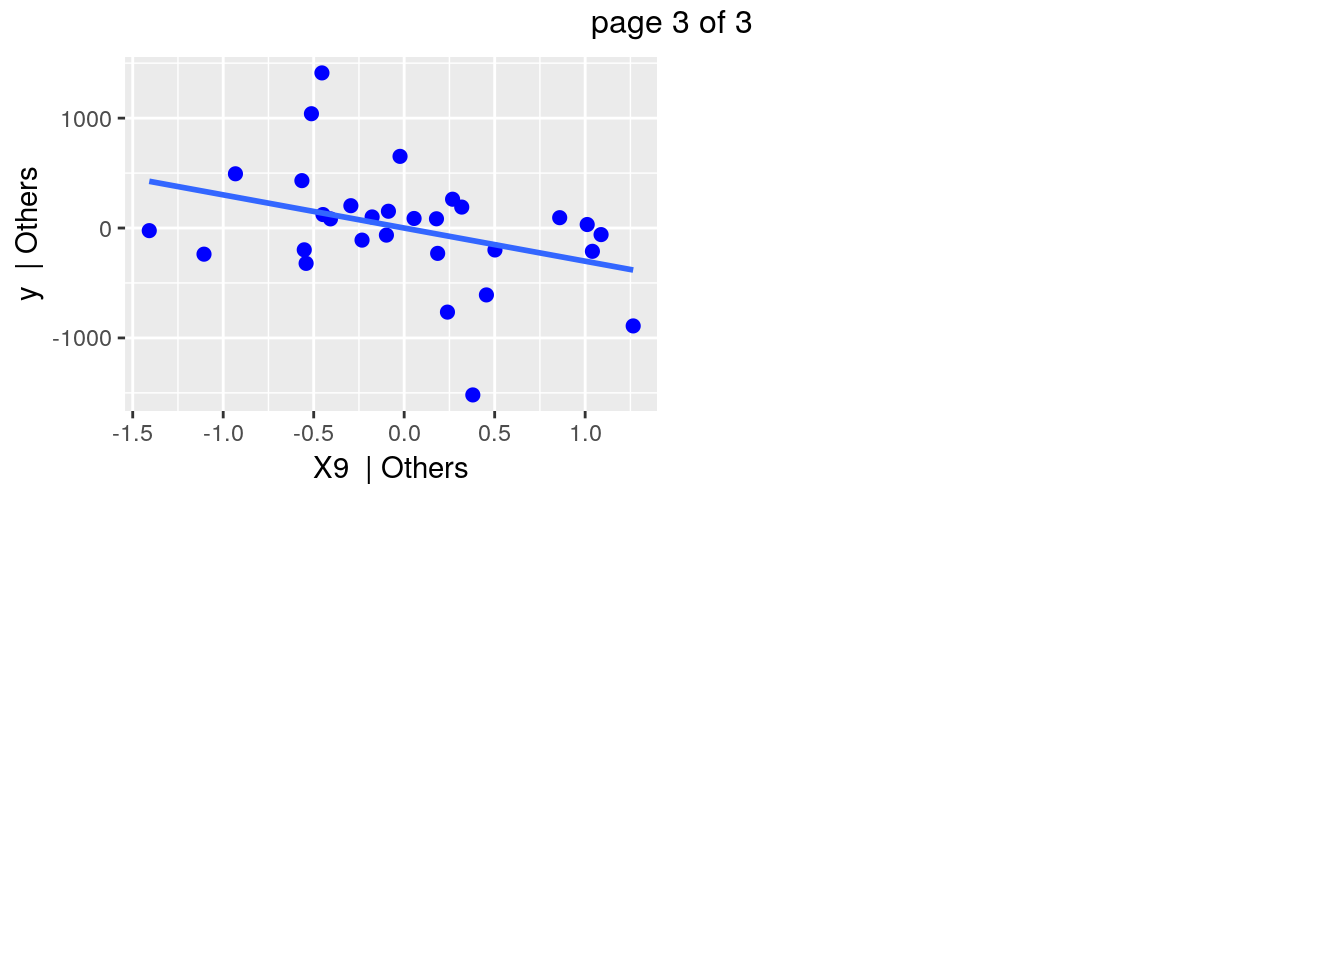
\includegraphics[width=0.25\linewidth]{lab6_stat565_files/figure-latex/unnamed-chunk-6-3}
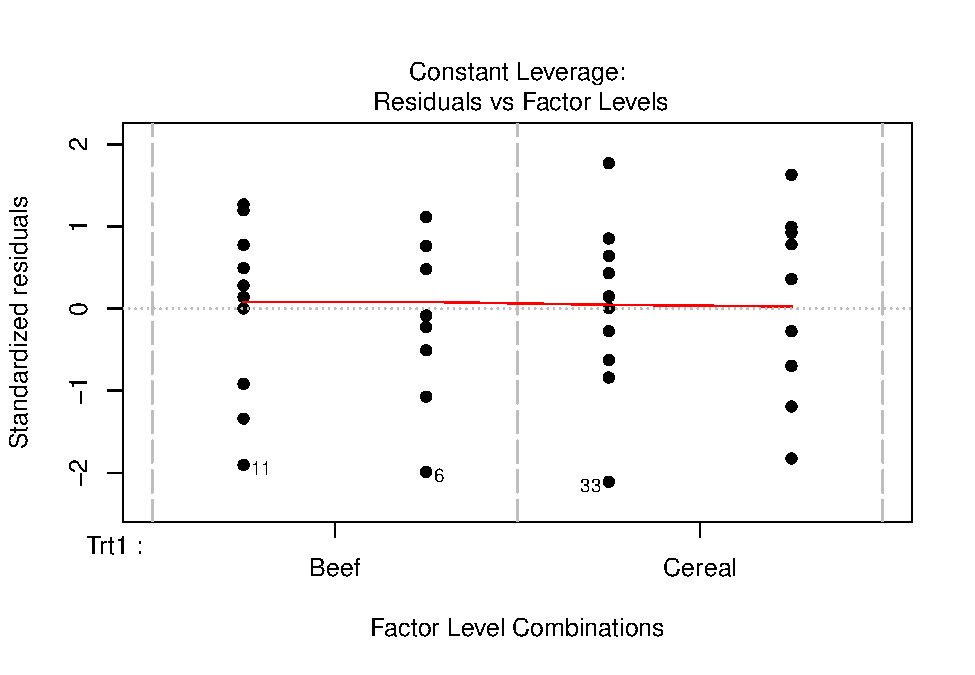
\includegraphics[width=0.25\linewidth]{lab6_stat565_files/figure-latex/unnamed-chunk-6-4}

\begin{enumerate}
\def\labelenumi{(\alph{enumi})}
\setcounter{enumi}{5}
\tightlist
\item
  \textcolor[rgb]{0.5,0.5,0.5}{Based on the residual plots, clearly explain whether assumptions in the model are satisfied or violated.}
\end{enumerate}

The plot of studentized residual versus predicted (fitted) value shows
that except few outliers, the residuals are evenly distributed about
zero at each prededict value (zero mean) and vertical deviations of
residuals from zero are about same for each predicted value (constant
variance).

The plots of studentized residual versus factor levels didn't show
obvious violation of zero mean and constant variance.

The QQ plot shows that some data points are not on the line and
flattening at the extremes, which is a litte violation of normality.

\begin{enumerate}
\def\labelenumi{(\alph{enumi})}
\setcounter{enumi}{6}
\tightlist
\item
  \textcolor[rgb]{0.5,0.5,0.5}{The researchers are interested in testing the following contrasts. Test each of the using software, and report conclusion along with p value.}
\end{enumerate}

c1
\textcolor[rgb]{0.5,0.5,0.5}{Mean yield for variety 1 versus variety 3 at method b}

The \(H0\) for contrast is
\(\mu_{b1.}-\mu_{b3.}=0\implies\beta_{1}-\beta_{3}+(\tau\beta)_{b1}-(\tau\beta)_{b3}=0\).
The \(H1\) is they don't equal zero.

The P-value of this contrast test is 0.8865, which is large enough. We
cannot reject the \(H0\) and conclude that the mean yield for variety 1
versus variety 3 at method b may be same at 5\% significance level. The
contrast tests with Boferroni or tukey's adjustment have the same
results (P-calue=1.0000, 0.9998, respectively).

c2
\textcolor[rgb]{0.5,0.5,0.5}{Mean yield for method a versus average of methods b and c}

The \(H0\) for contrast is
\(\mu_{a..}-\frac12(\mu_{b..}+\mu_{c..})=0\implies2\tau_a-\tau_b-\tau_c=0\).
The \(H1\) is they don't equal zero.

The P-value of this contrast test is 0.0000, which is small enough. We
can reject the \(H0\) and conclude that the mean yield for method a
versus average of methods b and c are significantly different at 5\%
significance level. The contrast tests with Boferroni or tukey's
adjustment have the same results (P-calue=0.0000, 0.0000, respectively).

c3
\textcolor[rgb]{0.5,0.5,0.5}{ Mean yield for method a versus average of methods b and c for variety 1}

The \(H0\) for contrast is \(\mu_{a1.}-\frac12(\mu_{b1.}+\mu_{c1.})=0\).
The \(H1\) is they don't equal zero.

The P-value of this contrast test is 0.0265, which is small enough. We
can reject the \(H0\) and conclude that the mean yield for method a
versus average of methods b and c for variety 1 are significantly
different at 5\% significance level. The contrast tests with Boferroni
or tukey's adjustment give the opposite results (P-calue=0.1060, 0.1019,
respectively).

c4
\textcolor[rgb]{0.5,0.5,0.5}{Mean yield for method a versus average of methods b and c between variety 1 and variety 2}

The \(H0\) for contrast is
\([\mu_{a1.}-\frac12(\mu_{b1.}+\mu_{c1.})]-[\mu_{a2.}-\frac12(\mu_{b2.}+\mu_{c2.})]=0\).
The \(H1\) is they don't equal zero.

The P-value of this contrast test is 0.5819, which is large enough. We
cannot reject the \(H0\) and conclude that the mean yield for method a
versus average of methods b and c for variety 1 may be same at 5\%
significance level. The contrast tests with Boferroni or tukey's
adjustment give the same results (P-calue=1.0000, 0.9694, respectively).

\begin{enumerate}
\def\labelenumi{(\alph{enumi})}
\setcounter{enumi}{7}
\tightlist
\item
  \textcolor[rgb]{0.5,0.5,0.5}{Report the code here without output.}
\end{enumerate}

\begin{Shaded}
\begin{Highlighting}[]
\NormalTok{table_grass <-}\StringTok{ }\KeywordTok{read_excel}\NormalTok{(}\StringTok{"Grass.xlsx"}\NormalTok{)}
\NormalTok{table_grass}\OperatorTok{$}\NormalTok{m <-}\StringTok{ }\KeywordTok{as.factor}\NormalTok{(table_grass}\OperatorTok{$}\NormalTok{method)}
\NormalTok{table_grass}\OperatorTok{$}\NormalTok{v <-}\StringTok{ }\KeywordTok{factor}\NormalTok{(table_grass}\OperatorTok{$}\NormalTok{variety, }\DataTypeTok{levels =} \KeywordTok{c}\NormalTok{(}\DecValTok{1}\NormalTok{, }\DecValTok{2}\NormalTok{, }\DecValTok{3}\NormalTok{, }\DecValTok{4}\NormalTok{, }\DecValTok{5}\NormalTok{), }\DataTypeTok{labels =} \KeywordTok{c}\NormalTok{(}\StringTok{"v1"}\NormalTok{, }
    \StringTok{"v2"}\NormalTok{, }\StringTok{"v3"}\NormalTok{, }\StringTok{"v4"}\NormalTok{, }\StringTok{"v5"}\NormalTok{))}
\NormalTok{table_grass}\OperatorTok{$}\NormalTok{mv <-}\StringTok{ }\KeywordTok{interaction}\NormalTok{(table_grass}\OperatorTok{$}\NormalTok{m, table_grass}\OperatorTok{$}\NormalTok{v)}
\NormalTok{model_grass <-}\StringTok{ }\KeywordTok{aov}\NormalTok{(y }\OperatorTok{~}\StringTok{ }\NormalTok{m }\OperatorTok{*}\StringTok{ }\NormalTok{v, }\DataTypeTok{data =}\NormalTok{ table_grass)}
\NormalTok{model_grass_inter <-}\StringTok{ }\KeywordTok{aov}\NormalTok{(y }\OperatorTok{~}\StringTok{ }\NormalTok{mv, }\DataTypeTok{data =}\NormalTok{ table_grass)}
\KeywordTok{str}\NormalTok{(table_grass)}
\KeywordTok{ggline}\NormalTok{(}\DataTypeTok{data =}\NormalTok{ table_grass, }\DataTypeTok{x =} \StringTok{"variety"}\NormalTok{, }\DataTypeTok{y =} \StringTok{"y"}\NormalTok{, }\DataTypeTok{add =} \KeywordTok{c}\NormalTok{(}\StringTok{"mean"}\NormalTok{, }\StringTok{"jitter"}\NormalTok{), }
    \DataTypeTok{shape =} \StringTok{"method"}\NormalTok{, }\DataTypeTok{color =} \StringTok{"method"}\NormalTok{, }\DataTypeTok{linetype =} \StringTok{"method"}\NormalTok{, }\DataTypeTok{ylab =} \StringTok{"y"}\NormalTok{, }\DataTypeTok{xlab =} \StringTok{"variety of table_grass"}\NormalTok{)}
\KeywordTok{pander}\NormalTok{(}\KeywordTok{favstats}\NormalTok{(y }\OperatorTok{~}\StringTok{ }\NormalTok{method, }\DataTypeTok{data =}\NormalTok{ table_grass))}
\KeywordTok{pander}\NormalTok{(}\KeywordTok{favstats}\NormalTok{(y }\OperatorTok{~}\StringTok{ }\NormalTok{method }\OperatorTok{|}\StringTok{ }\NormalTok{variety, }\DataTypeTok{data =}\NormalTok{ table_grass))}
\KeywordTok{summary}\NormalTok{(model_grass)}
\KeywordTok{plot}\NormalTok{(model_grass, }\DataTypeTok{pch =} \DecValTok{16}\NormalTok{)}

\CommentTok{# Test simple effects # Method-1# 1.1 Multiple comparison of levels in}
\CommentTok{# variety factor for a given level of method factor #}
\NormalTok{v_m <-}\StringTok{ }\KeywordTok{pairs}\NormalTok{(}\KeywordTok{lsmeans}\NormalTok{(}\DataTypeTok{object =}\NormalTok{ model_grass, }\DataTypeTok{specs =} \OperatorTok{~}\NormalTok{v }\OperatorTok{|}\StringTok{ }\NormalTok{m))}
\CommentTok{# 1.1 Multiple comparison of levels in method factor for a given level of}
\CommentTok{# variety factor #}
\NormalTok{m_v <-}\StringTok{ }\KeywordTok{pairs}\NormalTok{(}\KeywordTok{lsmeans}\NormalTok{(}\DataTypeTok{object =}\NormalTok{ model_grass, }\DataTypeTok{specs =} \OperatorTok{~}\NormalTok{m }\OperatorTok{|}\StringTok{ }\NormalTok{v))}
\CommentTok{# 1.1 same with}
\KeywordTok{lsmeans}\NormalTok{(model_grass, }\KeywordTok{list}\NormalTok{(pairwise }\OperatorTok{~}\StringTok{ }\NormalTok{v }\OperatorTok{|}\StringTok{ }\NormalTok{m, pairwise }\OperatorTok{~}\StringTok{ }\NormalTok{m }\OperatorTok{|}\StringTok{ }\NormalTok{v))}
\CommentTok{# 1.2 All the above Multiple comparisons with Tukey's adjustment # (strict)}
\KeywordTok{test}\NormalTok{(}\KeywordTok{rbind}\NormalTok{(v_m, m_v), }\DataTypeTok{adjust =} \StringTok{"tukey"}\NormalTok{)}

\CommentTok{# Test all the interaction effect# 1.}
\KeywordTok{pairs}\NormalTok{(}\KeywordTok{lsmeans}\NormalTok{(}\DataTypeTok{object =}\NormalTok{ model_grass, }\DataTypeTok{specs =} \OperatorTok{~}\NormalTok{v }\OperatorTok{+}\StringTok{ }\NormalTok{m))}
\KeywordTok{pairs}\NormalTok{(}\KeywordTok{lsmeans}\NormalTok{(}\DataTypeTok{object =}\NormalTok{ model_grass, }\DataTypeTok{specs =} \OperatorTok{~}\NormalTok{m }\OperatorTok{*}\StringTok{ }\NormalTok{v))}
\KeywordTok{pairs}\NormalTok{(}\KeywordTok{lsmeans}\NormalTok{(model_grass_inter, }\StringTok{"mv"}\NormalTok{))}
\KeywordTok{lsmeans}\NormalTok{(model_grass, pairwise }\OperatorTok{~}\StringTok{ }\NormalTok{v }\OperatorTok{+}\StringTok{ }\NormalTok{m)}
\KeywordTok{TukeyHSD}\NormalTok{(model_grass, }\DataTypeTok{conf.level =} \FloatTok{0.95}\NormalTok{)}
\KeywordTok{ScheffeTest}\NormalTok{(model_grass, }\DataTypeTok{conf.level =} \FloatTok{0.95}\NormalTok{)}
\CommentTok{# 2. another type of interaction effect}
\KeywordTok{contrast}\NormalTok{(}\KeywordTok{lsmeans}\NormalTok{(model_grass, }\OperatorTok{~}\NormalTok{v }\OperatorTok{*}\StringTok{ }\NormalTok{m), }\DataTypeTok{interaction =} \StringTok{"pairwise"}\NormalTok{)}

\CommentTok{# Test specific contrasts# 1. Create a inteaction variable by multiplying}
\CommentTok{# the two factors #}
\NormalTok{table_grass}\OperatorTok{$}\NormalTok{mv <-}\StringTok{ }\KeywordTok{interaction}\NormalTok{(table_grass}\OperatorTok{$}\NormalTok{m, table_grass}\OperatorTok{$}\NormalTok{v)}
\CommentTok{# 2. Fit the model again using only that new variable #}
\NormalTok{model_grass_inter <-}\StringTok{ }\KeywordTok{aov}\NormalTok{(y }\OperatorTok{~}\StringTok{ }\NormalTok{mv, }\DataTypeTok{data =}\NormalTok{ table_grass)}
\KeywordTok{summary}\NormalTok{(model_grass_inter)  }\CommentTok{# Check the ANOVA#}
\KeywordTok{summary.lm}\NormalTok{(model_grass_inter)  }\CommentTok{# Check the estimated model coefficients. Same with previous#}

\CommentTok{# 2. Obtain least square estimates for treatment combinations #}
\NormalTok{lsmf_grass <-}\StringTok{ }\KeywordTok{lsmeans}\NormalTok{(model_grass_inter, }\StringTok{"mv"}\NormalTok{)}

\CommentTok{# 2. Check the order of terms# 3. Write the vectors of contrasts#}
\NormalTok{contrast_list_grass <-}\StringTok{ }\KeywordTok{list}\NormalTok{(}\DataTypeTok{b1_b3 =} \KeywordTok{c}\NormalTok{(}\DecValTok{0}\NormalTok{, }\DecValTok{1}\NormalTok{, }\KeywordTok{rep}\NormalTok{(}\DecValTok{0}\NormalTok{, }\DecValTok{5}\NormalTok{), }\DecValTok{-1}\NormalTok{, }\KeywordTok{rep}\NormalTok{(}\DecValTok{0}\NormalTok{, }\DecValTok{7}\NormalTok{)), }\DataTypeTok{a_b.c =} \KeywordTok{c}\NormalTok{(}\KeywordTok{rep}\NormalTok{(}\KeywordTok{c}\NormalTok{(}\DecValTok{1}\NormalTok{, }
    \FloatTok{-0.5}\NormalTok{, }\FloatTok{-0.5}\NormalTok{), }\DecValTok{5}\NormalTok{)}\OperatorTok{/}\DecValTok{5}\NormalTok{), }\DataTypeTok{a1_b1.c1 =} \KeywordTok{c}\NormalTok{(}\DecValTok{1}\NormalTok{, }\FloatTok{-0.5}\NormalTok{, }\FloatTok{-0.5}\NormalTok{, }\KeywordTok{rep}\NormalTok{(}\DecValTok{0}\NormalTok{, }\DecValTok{12}\NormalTok{)), }\DataTypeTok{a1_b1.c1__a1_b1.c1 =} \KeywordTok{c}\NormalTok{(}\DecValTok{1}\NormalTok{, }
    \FloatTok{-0.5}\NormalTok{, }\FloatTok{-0.5}\NormalTok{, }\DecValTok{0}\NormalTok{, }\DecValTok{0}\NormalTok{, }\DecValTok{0}\NormalTok{, }\DecValTok{-1}\NormalTok{, }\FloatTok{0.5}\NormalTok{, }\FloatTok{0.5}\NormalTok{, }\KeywordTok{rep}\NormalTok{(}\DecValTok{0}\NormalTok{, }\DecValTok{6}\NormalTok{)))}
\CommentTok{# Variety 1 versus Variety 3 at Method b # Method a versus average of}
\CommentTok{# Methods b and c averaged across Varieties. # Method a versus average of}
\CommentTok{# Methods b and c for Variety 1 # Method a versus average of Methods b and c}
\CommentTok{# between Variety 1 and Variety 2 #}

\KeywordTok{contrast}\NormalTok{(lsmf_grass, contrast_list_grass)  }\CommentTok{# without adjustment #}
\KeywordTok{summary}\NormalTok{(}\KeywordTok{contrast}\NormalTok{(lsmf_grass, contrast_list_grass), }\DataTypeTok{adjust =} \StringTok{"bonferroni"}\NormalTok{)  }\CommentTok{# Bonferroni#}
\KeywordTok{summary}\NormalTok{(}\KeywordTok{contrast}\NormalTok{(lsmf_grass, contrast_list_grass), }\DataTypeTok{adjust =} \StringTok{"tukey"}\NormalTok{)  }\CommentTok{#Tukey's#}
\end{Highlighting}
\end{Shaded}


\end{document}
